%\chapter{Something}\label{sec:something}

%Blah, blah \dots

% \cleardoublepage


\chapter{Additional TC Genesis Plots}\label{sec:genesis-appendix}

\begin{figure}[ht]
	\centering
	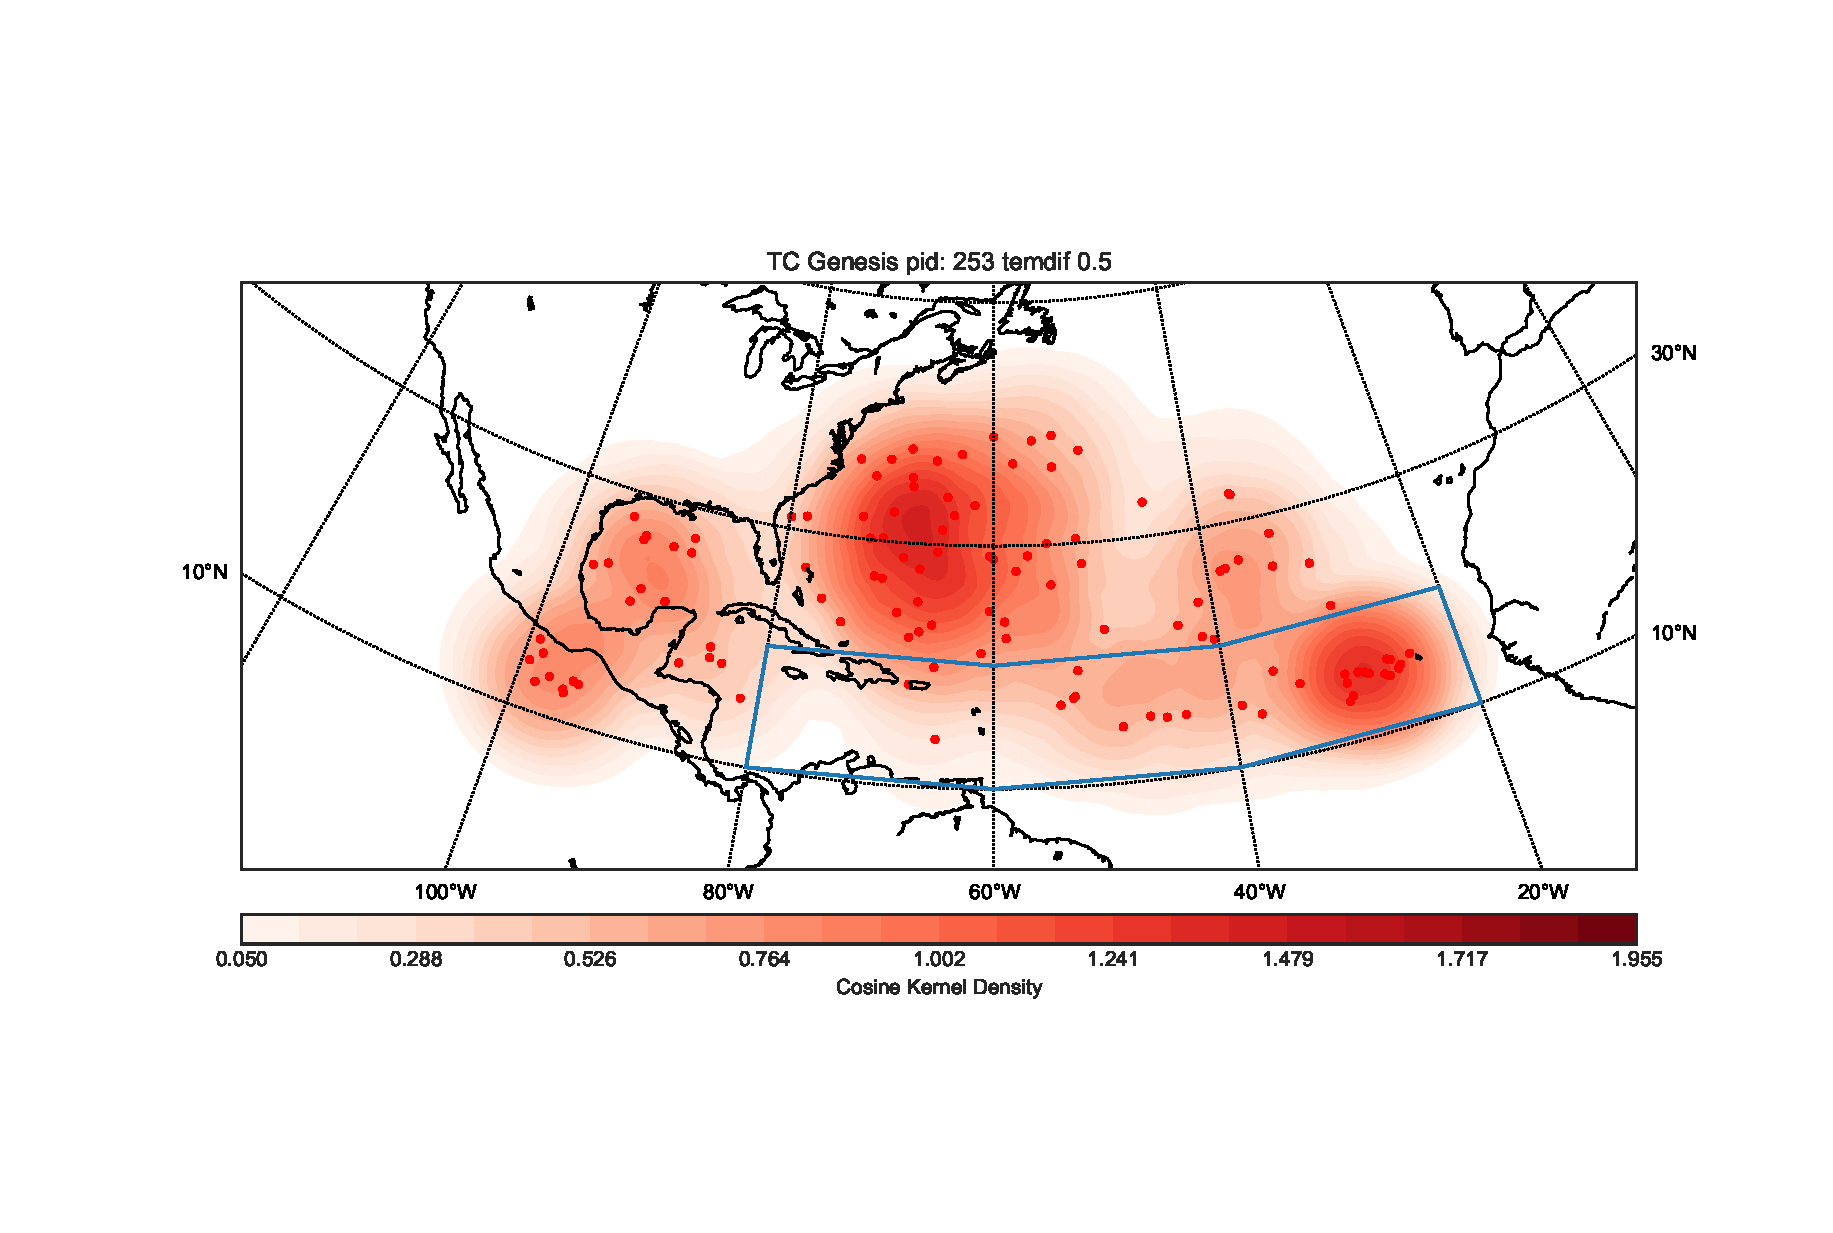
\includegraphics[width=0.7\textwidth]{img/genesis_plot_temdif05.eps}
	\caption{Genesis spots and density for a specific parameter combination.}
\end{figure}
\begin{figure}[ht]
	\centering
	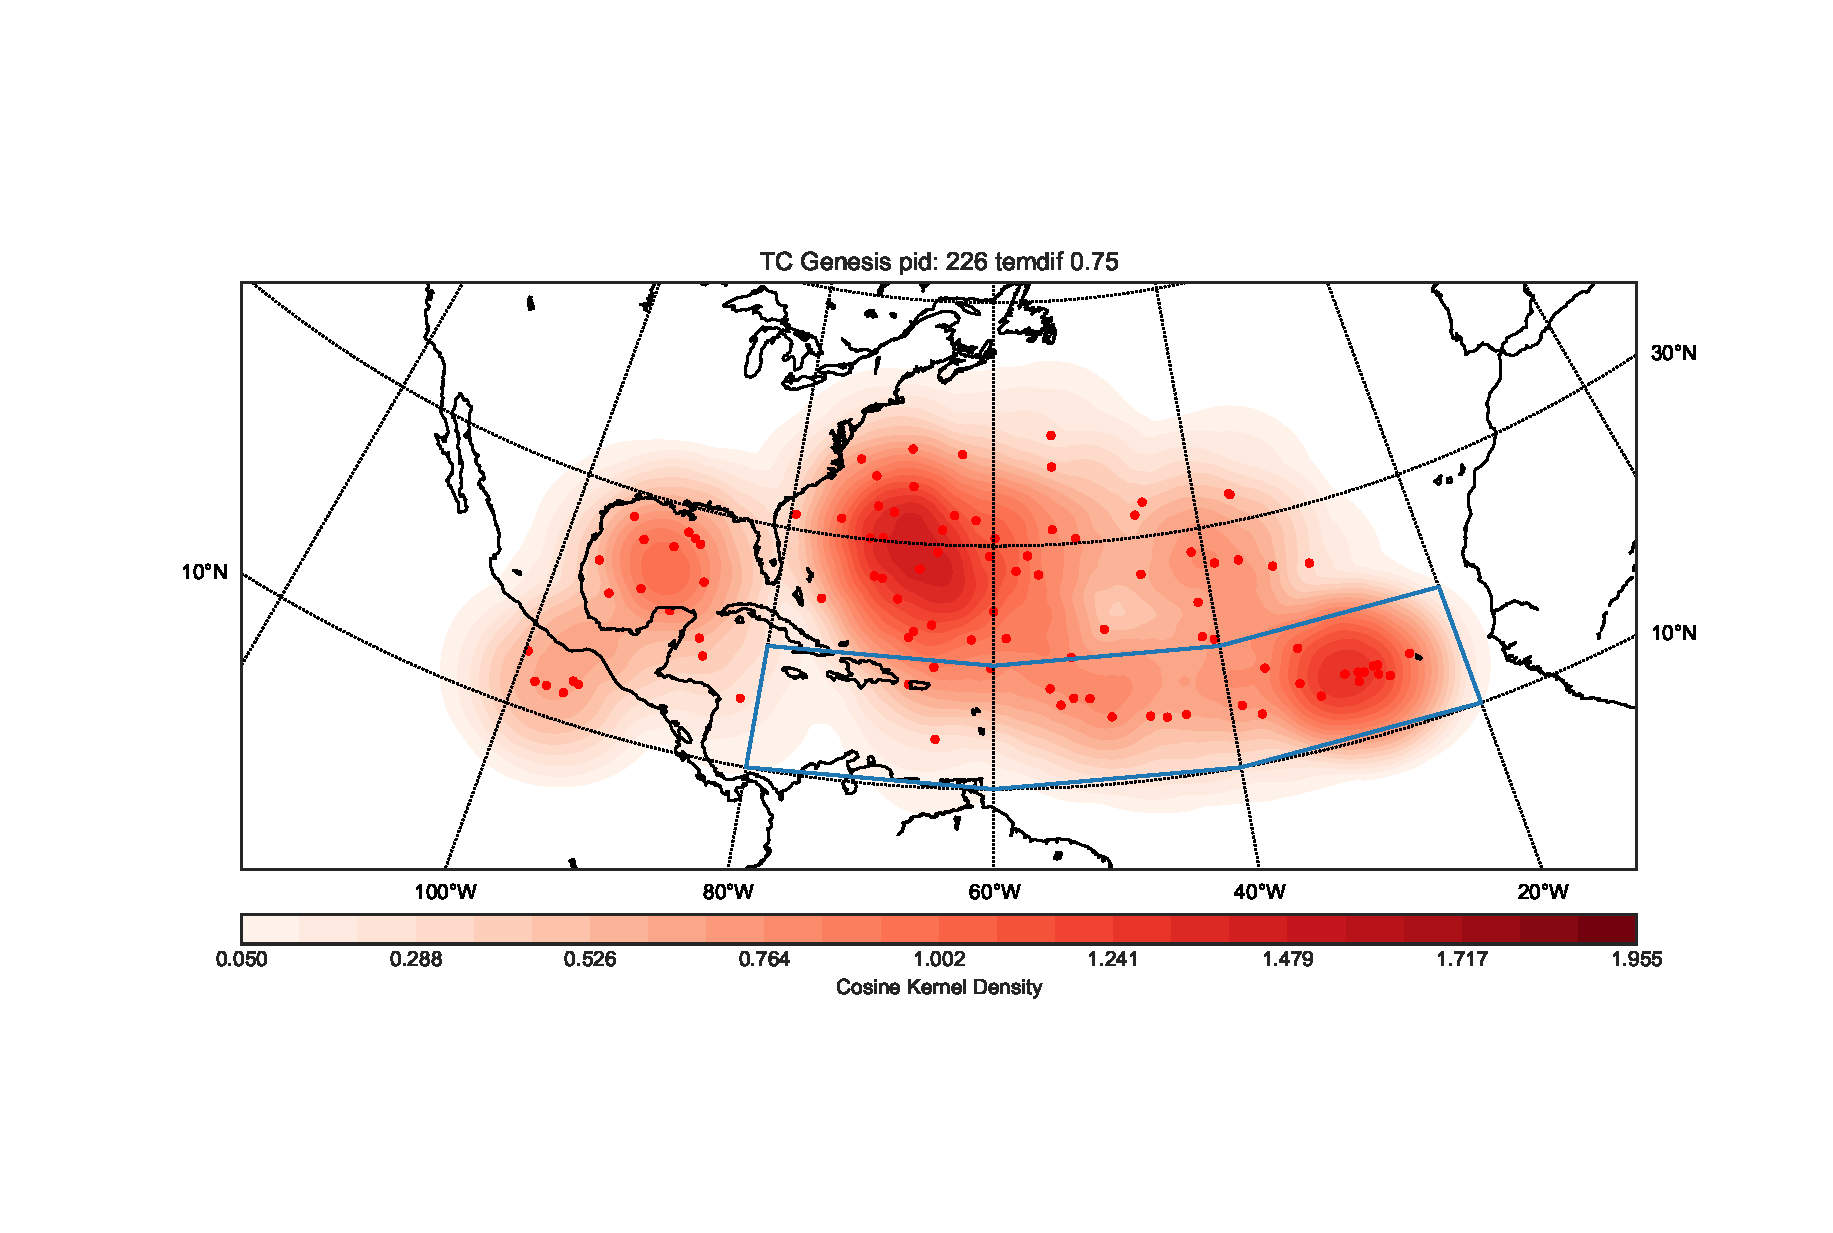
\includegraphics[width=0.7\textwidth]{img/genesis_plot_temdif075.eps}
	\caption{Genesis spots and density for a specific parameter combination.}
\end{figure}
\begin{figure}[ht]
	\centering
	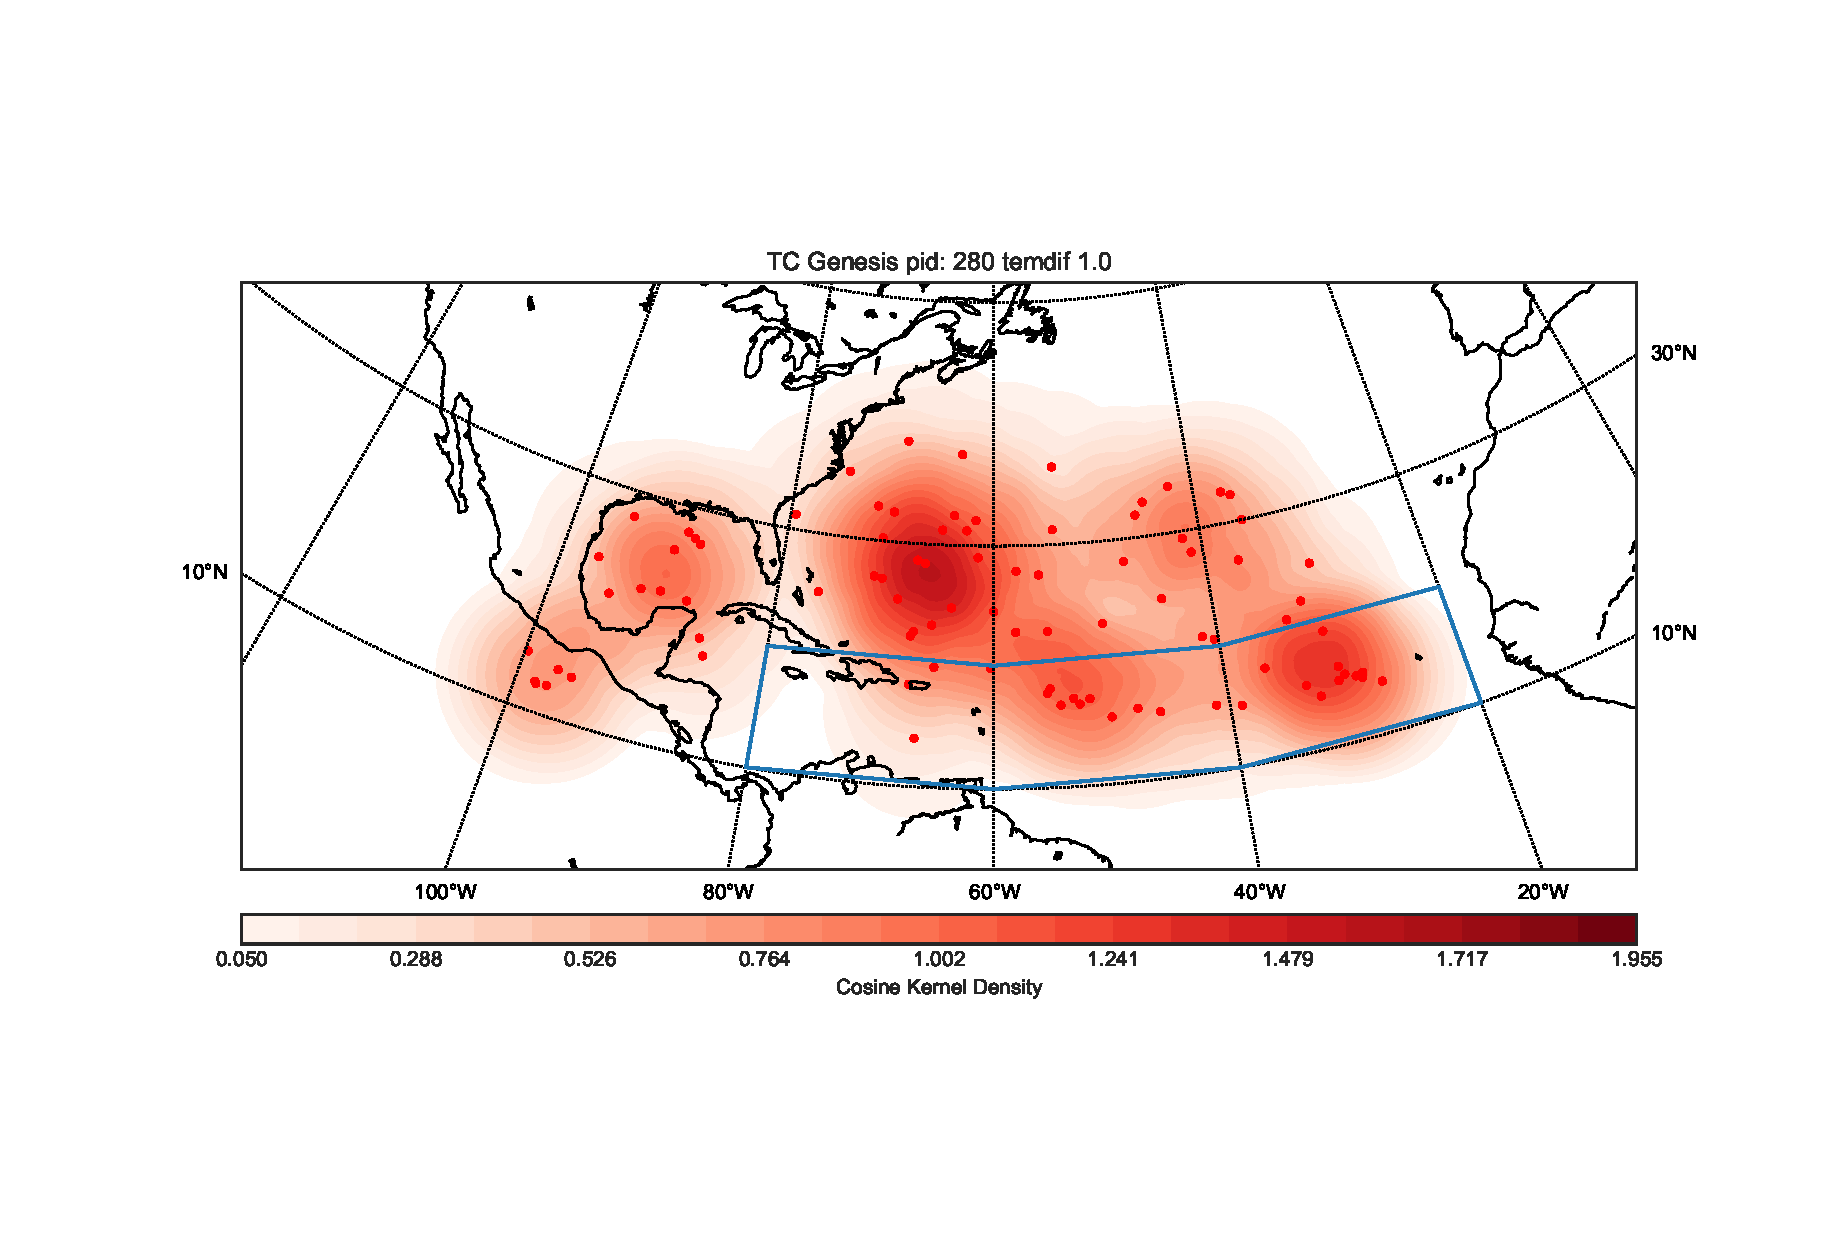
\includegraphics[width=0.7\textwidth]{img/genesis_plot_temdif1.eps}
	\caption{Genesis spots and density for a specific parameter combination.}
\end{figure}
\begin{figure}[ht]
	\centering
	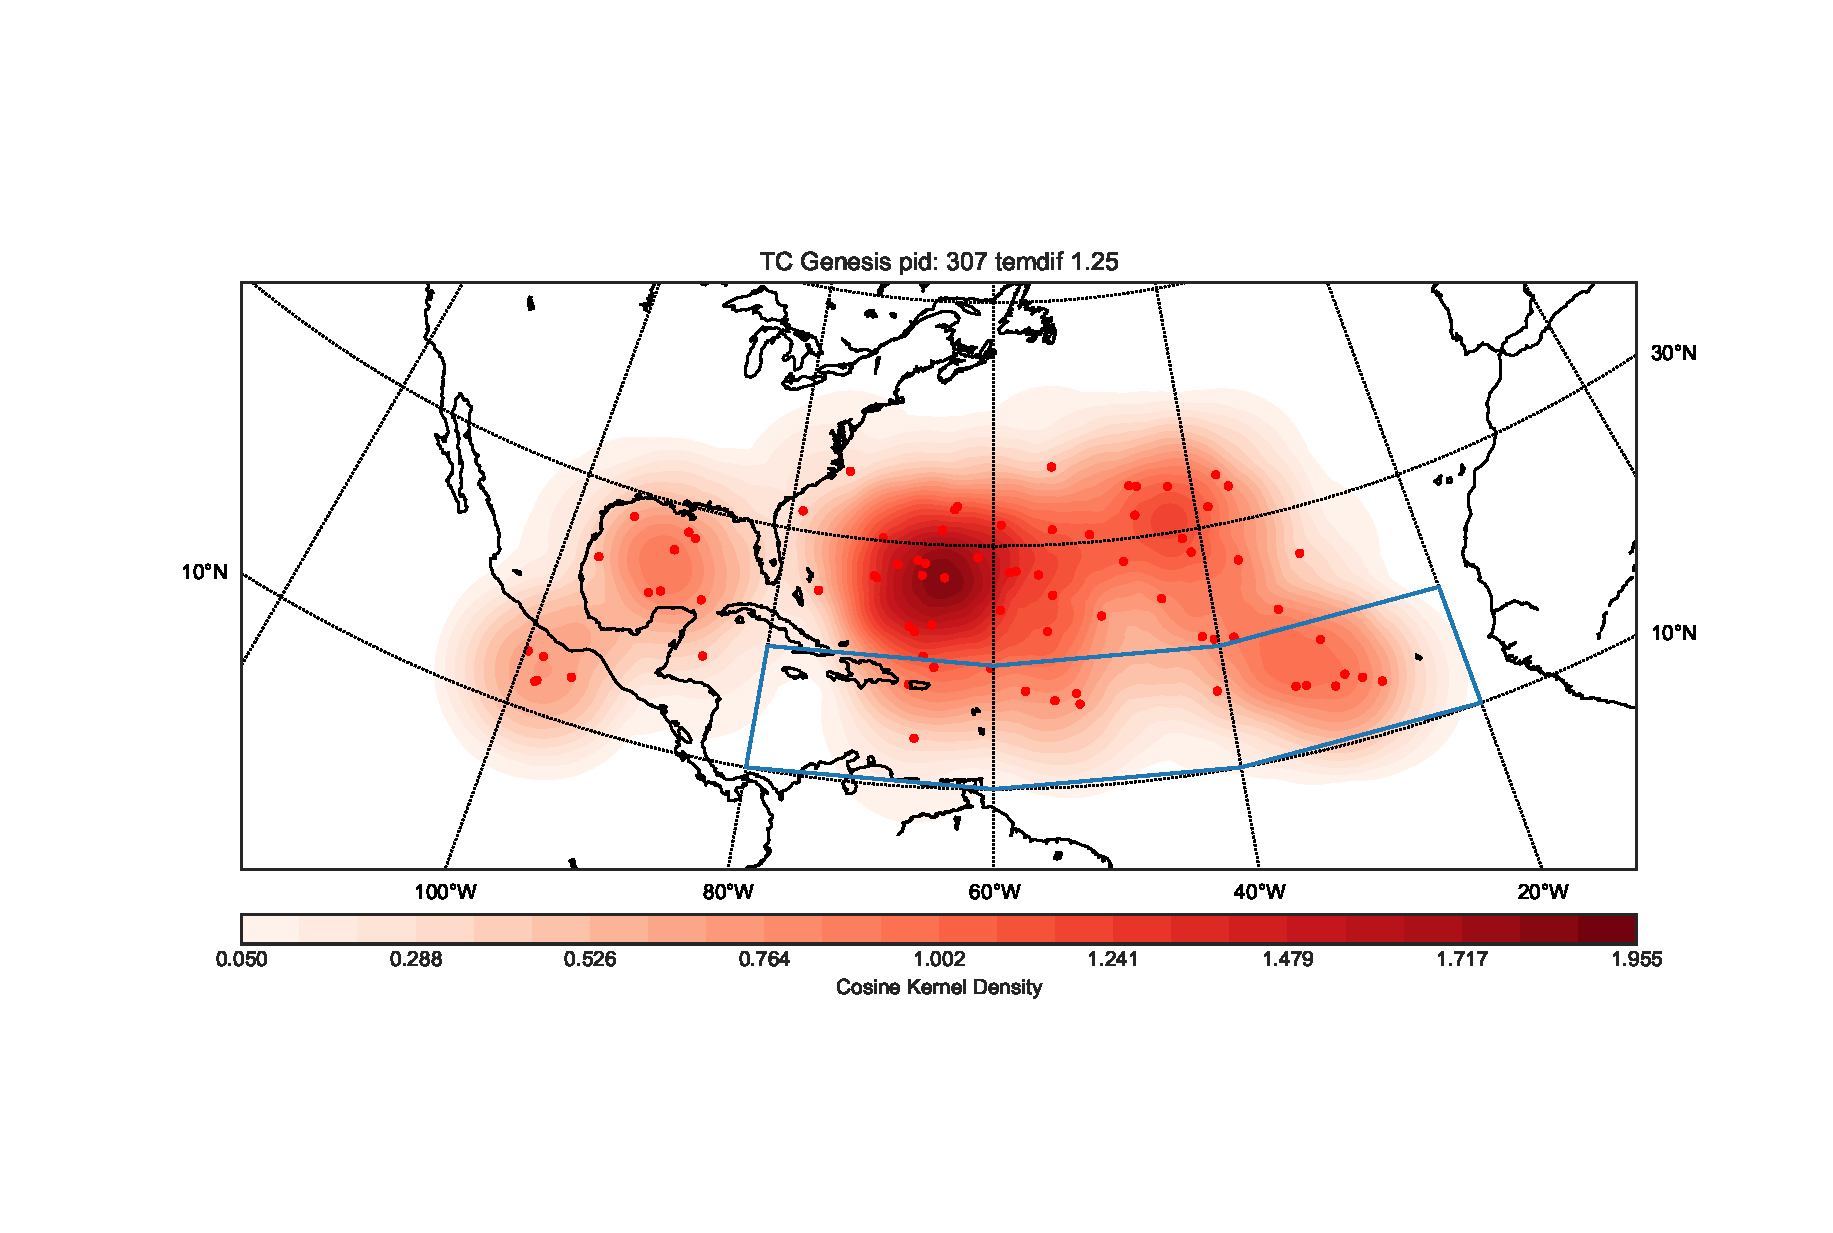
\includegraphics[width=0.7\textwidth]{img/genesis_plot_temdif125.eps}
	\caption{Genesis spots and density for a specific parameter combination.}
\end{figure}
\begin{figure}[ht]
	\centering
	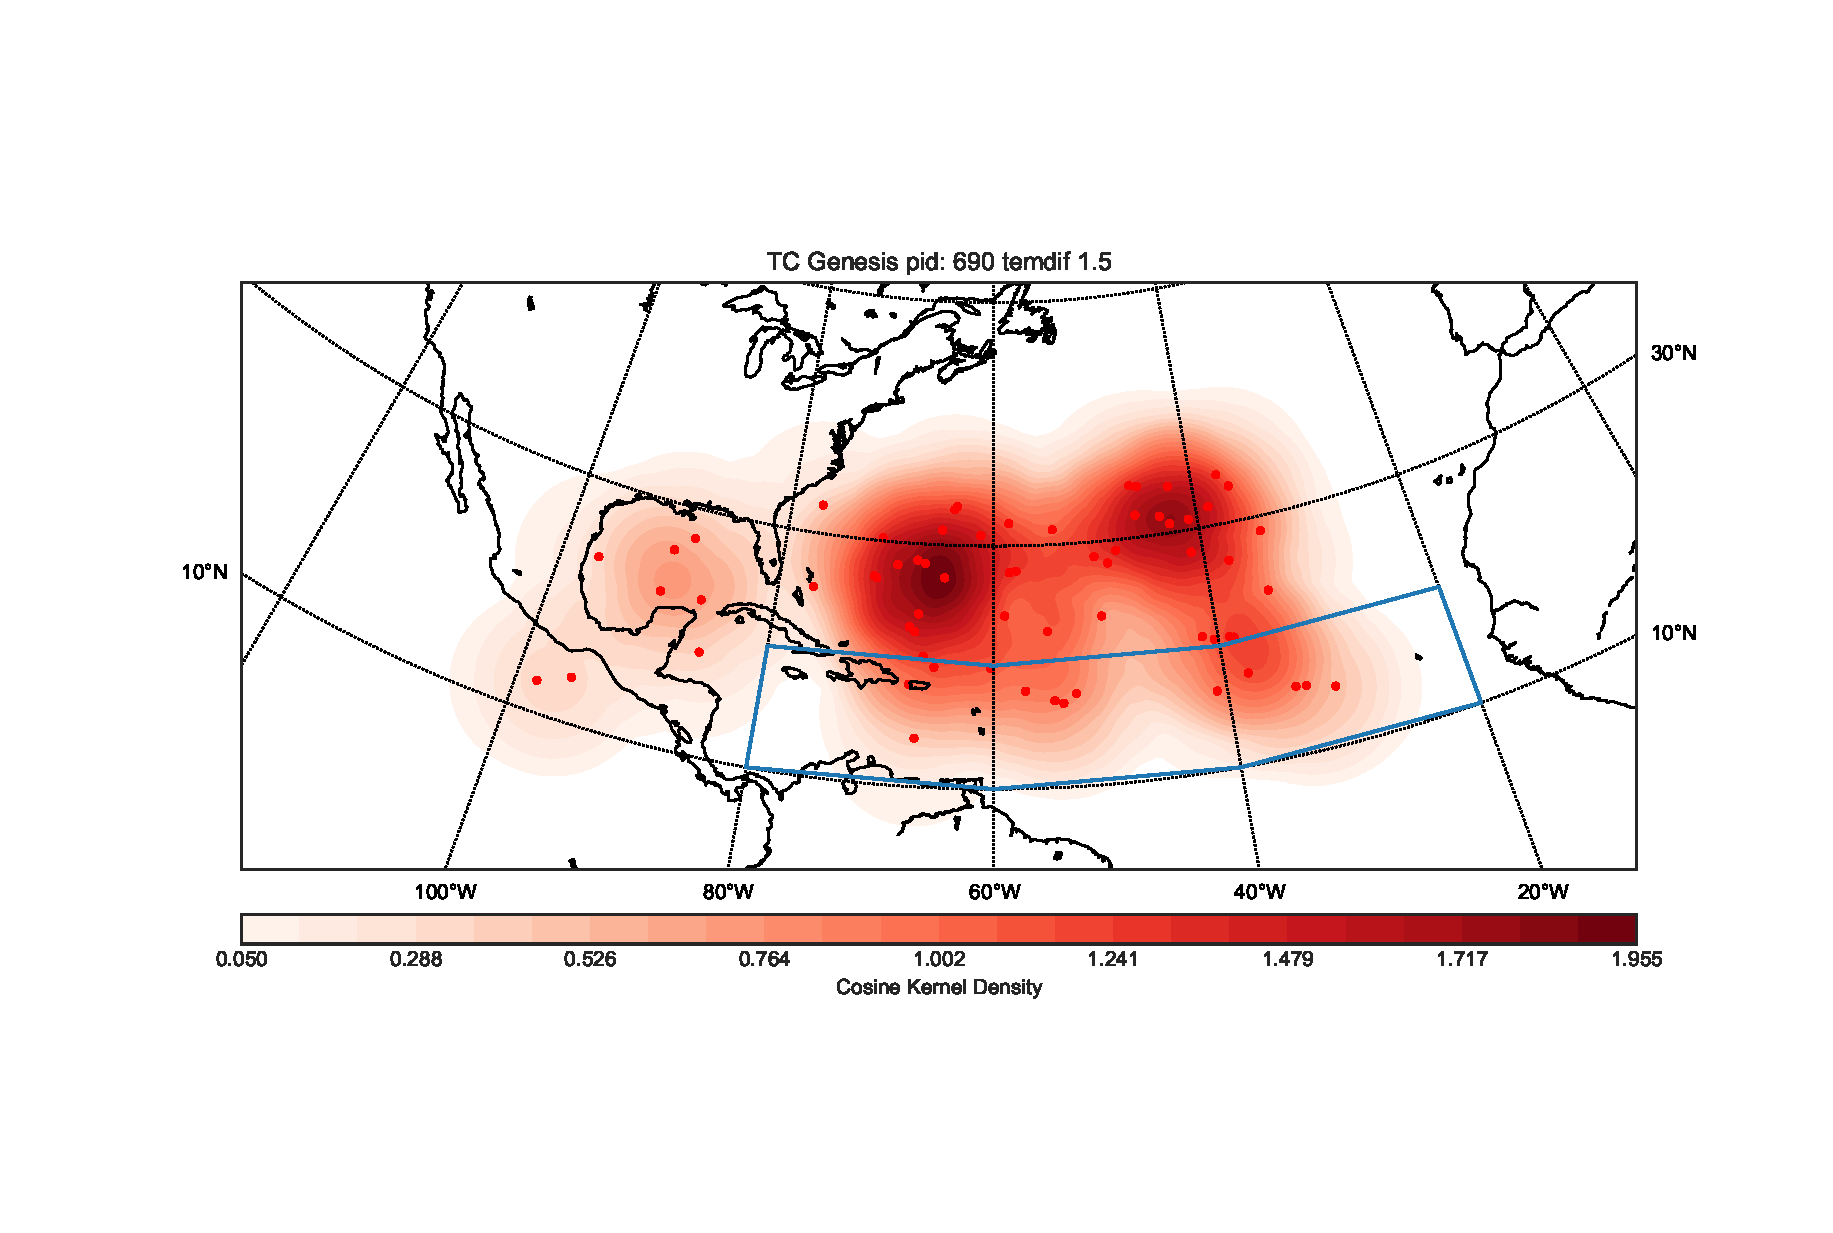
\includegraphics[width=0.7\textwidth]{img/genesis_plot_temdif15.eps}
	\caption{Genesis spots and density for a specific parameter combination.}
\end{figure}
 \cleardoublepage
 
%---------------------------------------------------------------------------
% Symbols

\chapter*{Nomenclature}\label{chap:symbole}
 \addcontentsline{toc}{chapter}{Nomenclature}
 
 \section*{Symbols}
\begin{tabbing}
 \hspace*{1.6cm} \= \hspace*{8cm} \= \kill
 $\mathrm{EHC}$ \> Conditional equation \> [$-$] \\[0.5ex]
 $e$ \> Willans coefficient \> [$-$] \\[0.5ex]
 $F,G$ \> Parts of the system equation \> [\unitfrac[]{K}{s}]
\end{tabbing}

\section*{Indicies}
\begin{tabbing}
 \hspace*{1.6cm}  \= \kill
 a \> Ambient \\[0.5ex]
 air \> Air
\end{tabbing}

\section*{Acronyms and Abbreviations}
\begin{tabbing}
 \hspace*{1.6cm}  \= \kill
 ETH \> Eidgen\"{o}ssische Technische Hochschule \\[0.5ex]
 TC \> Tropical Cyclone \\[0.5ex]
 DWD \> German Weather Service\\[0.5ex]
 MPIM \> Max Planck Institute for Meteorology\\[0.5ex]
ICON \> Icosahedral Nonhydrostatic Model developed by the DWD and the
MPIM\\[0.5ex]
SST \> sea surface temperature\\[0.5ex]
SLP \> sea level pressure\\[0.5ex]
MDR \> main development region  \\[0.5ex]
\end{tabbing}

%---------------------------------------------------------------------------
